% Diego Sebastián Aliaga Damián
% 2024200481M
% Tema 96: Fintech y financiamiento participativo (crowdfunding) en el Perú: oferta y condiciones
% Póster del artículo (consigna 2.2, «Contenido del póster»: título, autor del artículo, autor del póster, contexto,
% problema, objetivo, metodología, resultados, conclusiones, fuente de datos y QR del repositorio de extracción).
% Mismo diseño que los pósteres de los artículos del estado del arte (verde y oro de la UNCP), en A0.
% Las cifras usan \cifra{...} (articulo/generado/cifras.tex) y las figuras salen de salidas/figuras (04_analisis.py).
% BORRADOR ASISTIDO POR IA (2026-11-12): revisar y ajustar el texto con tus palabras.
% Compilación: python ../../herramientas/productos/compilar_productos.py
\documentclass[fontsize=27pt,parskip=half-]{scrartcl}
\usepackage[paperwidth=841mm,paperheight=1189mm,left=32mm,right=32mm,top=28mm,bottom=24mm]{geometry}
\usepackage[T1]{fontenc}
\usepackage[utf8]{inputenc}
\usepackage[spanish,es-noshorthands,es-nodecimaldot,es-tabla]{babel}
\usepackage{tgheros}
\renewcommand{\familydefault}{\sfdefault}
\usepackage{anyfontsize,xcolor,graphicx,booktabs,tabularx,multicol,enumitem,qrcode,ragged2e,csquotes}
\usepackage{tikz}
\usetikzlibrary{calc}
\usepackage[most]{tcolorbox}
\usepackage{caption}
\usepackage{newunicodechar}
\newunicodechar{≤}{\ensuremath{\leq}}
\newunicodechar{−}{\ensuremath{-}}
\usepackage[style=apa,backend=biber]{biblatex}
\addbibresource{../../articulo/referencias.bib}
\usepackage{xurl}
\urlstyle{same}

% Generado por herramientas/articulo/generar_insumos_articulo.py; no editar a mano.
\newcommand{\cifra}[1]{\ifcsname cifra@#1\endcsname\csname cifra@#1\endcsname\else\textbf{??#1??}\fi}
\expandafter\def\csname cifra@acfPrevia\endcsname{0.84}
\expandafter\def\csname cifra@bootstrap\endcsname{10\,000}
\expandafter\def\csname cifra@coberturaPct\endcsname{90.3}
\expandafter\def\csname cifra@colocacion2022\endcsname{54.5}
\expandafter\def\csname cifra@colocacion2023\endcsname{77.9}
\expandafter\def\csname cifra@colocacion2024\endcsname{83.4}
\expandafter\def\csname cifra@colocacion2025\endcsname{88.5}
\expandafter\def\csname cifra@colocacion2026\endcsname{94.2}
\expandafter\def\csname cifra@colocacionEmp\endcsname{89.5}
\expandafter\def\csname cifra@colocacionPer\endcsname{51.4}
\expandafter\def\csname cifra@columnasPanel\endcsname{35}
\expandafter\def\csname cifra@costoAcumulada\endcsname{0.76}
\expandafter\def\csname cifra@costoMediana\endcsname{5.27}
\expandafter\def\csname cifra@costoTrimestres\endcsname{17}
\expandafter\def\csname cifra@cotaMaxAnual\endcsname{0.22}
\expandafter\def\csname cifra@cotaPctMax\endcsname{1.7}
\expandafter\def\csname cifra@cotaPctMaxDesde2024\endcsname{0.2}
\expandafter\def\csname cifra@crecMensualPrevio\endcsname{8.9}
\expandafter\def\csname cifra@eUnoN\endcsname{8}
\expandafter\def\csname cifra@eUnoPMin\endcsname{0.116}
\expandafter\def\csname cifra@eUnoRhoMax\endcsname{0.01}
\expandafter\def\csname cifra@eUnoRhoMin\endcsname{-0.22}
\expandafter\def\csname cifra@eeffEscala\endcsname{8}
\expandafter\def\csname cifra@eeffEscalaCorregida\endcsname{3}
\expandafter\def\csname cifra@eeffEscalaExcluida\endcsname{5}
\expandafter\def\csname cifra@fechaCorte\endcsname{septiembre de 2026}
\expandafter\def\csname cifra@fechaInicio\endcsname{enero de 2021}
\expandafter\def\csname cifra@filasPanel\endcsname{414}
\expandafter\def\csname cifra@hDosFisherOR\endcsname{2.84}
\expandafter\def\csname cifra@hDosFisherP\endcsname{0.127}
\expandafter\def\csname cifra@hDosP\endcsname{< 0.001}
\expandafter\def\csname cifra@hDosZ\endcsname{14.88}
\expandafter\def\csname cifra@hUnoICinf\endcsname{5.63}
\expandafter\def\csname cifra@hUnoICsup\endcsname{11.27}
\expandafter\def\csname cifra@hUnoMedianaAntes\endcsname{3.32}
\expandafter\def\csname cifra@hUnoMedianaDespues\endcsname{11.37}
\expandafter\def\csname cifra@hUnoNAntes\endcsname{42}
\expandafter\def\csname cifra@hUnoNDespues\endcsname{10}
\expandafter\def\csname cifra@hUnoP\endcsname{< 0.001}
\expandafter\def\csname cifra@hUnoPCota\endcsname{< 0.001}
\expandafter\def\csname cifra@hUnoPSinLider\endcsname{0.124}
\expandafter\def\csname cifra@hUnoU\endcsname{387}
\expandafter\def\csname cifra@hhi2022\endcsname{8\,882}
\expandafter\def\csname cifra@hhi2023\endcsname{9\,770}
\expandafter\def\csname cifra@hhi2024\endcsname{9\,999}
\expandafter\def\csname cifra@hhi2025\endcsname{9\,977}
\expandafter\def\csname cifra@hhi2026\endcsname{9\,321}
\expandafter\def\csname cifra@inicioFPF\endcsname{junio de 2022}
\expandafter\def\csname cifra@interanualAntes\endcsname{169}
\expandafter\def\csname cifra@interanualDespues\endcsname{27}
\expandafter\def\csname cifra@interanualP\endcsname{1.000}
\expandafter\def\csname cifra@lider\endcsname{Inversiones.io}
\expandafter\def\csname cifra@mesesActividadFPF\endcsname{52}
\expandafter\def\csname cifra@mesesDespues\endcsname{10}
\expandafter\def\csname cifra@mesesObtenidos\endcsname{374}
\expandafter\def\csname cifra@mesesSobreTendencia\endcsname{0}
\expandafter\def\csname cifra@monto2022\endcsname{6.46}
\expandafter\def\csname cifra@monto2023\endcsname{16.24}
\expandafter\def\csname cifra@monto2024\endcsname{54.28}
\expandafter\def\csname cifra@monto2025\endcsname{120.28}
\expandafter\def\csname cifra@monto2026\endcsname{104.71}
\expandafter\def\csname cifra@montoMedio2022\endcsname{58.8}
\expandafter\def\csname cifra@montoMedio2023\endcsname{115.2}
\expandafter\def\csname cifra@montoMedio2024\endcsname{215.4}
\expandafter\def\csname cifra@montoMedio2025\endcsname{278.4}
\expandafter\def\csname cifra@montoMedio2026\endcsname{320.2}
\expandafter\def\csname cifra@montoTotal\endcsname{301.97}
\expandafter\def\csname cifra@noObtenidos\endcsname{40}
\expandafter\def\csname cifra@noObtenidosVentana\endcsname{28}
\expandafter\def\csname cifra@participacionLider\endcsname{98.5}
\expandafter\def\csname cifra@pctEmpresarialPrincipal\endcsname{99.5}
\expandafter\def\csname cifra@pctPersonalPrincipal\endcsname{95.3}
\expandafter\def\csname cifra@perLiderFin\endcsname{9}
\expandafter\def\csname cifra@perLiderPub\endcsname{12}
\expandafter\def\csname cifra@placeboN\endcsname{5}
\expandafter\def\csname cifra@placeboPMax\endcsname{< 0.001}
\expandafter\def\csname cifra@plataformasAutorizadas\endcsname{6}
\expandafter\def\csname cifra@plataformasConFinanciamiento\endcsname{3}
\expandafter\def\csname cifra@plataformasVigentes\endcsname{3}
\expandafter\def\csname cifra@principalPersonal\endcsname{Afluenta}
\expandafter\def\csname cifra@proyFin2022\endcsname{110}
\expandafter\def\csname cifra@proyFin2023\endcsname{141}
\expandafter\def\csname cifra@proyFin2024\endcsname{252}
\expandafter\def\csname cifra@proyFin2025\endcsname{432}
\expandafter\def\csname cifra@proyFin2026\endcsname{327}
\expandafter\def\csname cifra@proyFinTotal\endcsname{1\,262}
\expandafter\def\csname cifra@rDosTendencia\endcsname{0.81}
\expandafter\def\csname cifra@saltoTEA\endcsname{19.2}
\expandafter\def\csname cifra@semilla\endcsname{0481}
\expandafter\def\csname cifra@solicitudesDiagnostico\endcsname{26}
\expandafter\def\csname cifra@solicitudesHTTP\endcsname{1\,702}
\expandafter\def\csname cifra@solicitudesHTTPok\endcsname{1\,702}
\expandafter\def\csname cifra@varMonto2023\endcsname{151.3}
\expandafter\def\csname cifra@varMonto2024\endcsname{234.3}
\expandafter\def\csname cifra@varMonto2025\endcsname{121.6}
\expandafter\def\csname cifra@varMonto2026\endcsname{14.7}

\graphicspath{{../../salidas/figuras/}{../posteres_articulos/img/}}
\newcommand{\repositorio}{https://github.com/Diego-Aliaga-Damian/finanzas1-u2-crowdfunding-peru}

\definecolor{primario}{HTML}{0A5C1F}
\definecolor{primarioclaro}{HTML}{E5F1E2}
\definecolor{ola}{HTML}{7DB878}
\definecolor{oro}{HTML}{F8D008}
\definecolor{acento}{HTML}{B8900A}
\definecolor{tinta}{HTML}{1B1B1B}
\definecolor{gris}{HTML}{9A9A9A}
\color{tinta}
\pagestyle{empty}
\setlength{\parindent}{0pt}
\setlength{\columnsep}{24mm}
\setlist[itemize]{label={\color{acento}\textbullet}, leftmargin=1.1em, itemsep=0.3em, topsep=0.3em}
\setlist[enumerate]{leftmargin=1.4em, itemsep=0.3em, topsep=0.3em}
\captionsetup{font=small, labelfont=bf, labelsep=colon, justification=centering, skip=6pt}
\newcommand{\singuiones}{\raggedright\hyphenpenalty=10000\exhyphenpenalty=10000}
\newcounter{seccion}
\newcommand{\seccion}[1]{\par\vspace{0.8em}{\color{gris}\hrule height 1.2pt}\vspace{0.7em}%
  \refstepcounter{seccion}{\singuiones\color{primario}\bfseries\fontsize{44}{51}\selectfont\theseccion.\hspace{0.45em}#1\par}\vspace{0.4em}}
\newcommand{\dato}[1]{{\color{primario}\bfseries #1}}

\begin{document}
% Ondas decorativas junto al título
\begin{tikzpicture}[remember picture,overlay]
  \begin{scope}[shift={($(current page.north east)+(-30cm,-38cm)$)}]
    \foreach \k in {0,...,48}{
      \draw[ola!85, line width=0.8pt] plot[domain=0:29, samples=150, smooth]
        (\x, {2.0*sin(\x*20 + \k*6) + 1.0*sin(\x*8 - \k*5) + \k*0.16});
    }
  \end{scope}
\end{tikzpicture}%
% ---------- Encabezado institucional ----------
\begin{minipage}[c]{0.09\linewidth}
\includegraphics[width=\linewidth]{logo_uncp.png}\end{minipage}\hspace{1.2em}%
\begin{minipage}[c]{0.36\linewidth}
  {\color{primario}\bfseries\fontsize{58}{67}\selectfont Universidad Nacional\\del Centro del Perú\par}
\end{minipage}\hspace{1em}%
\begin{minipage}[c]{0.40\linewidth}
  {\bfseries\fontsize{40}{47}\selectfont Facultad de Economía\par}
  {\fontsize{31}{37}\selectfont Escuela Profesional de Economía · Finanzas I (055D), Unidad II\par}
\end{minipage}\hfill
\begin{minipage}[c]{0.085\linewidth}\raggedleft
\includegraphics[width=\linewidth]{logo_facultad.png}\end{minipage}

\vspace{1cm}
{\color{oro}\rule{\linewidth}{8pt}}
\vspace{1.6cm}

% ---------- Título y autoría ----------
\begin{minipage}[t]{0.68\linewidth}
  {\singuiones\color{primario}\bfseries\fontsize{84}{98}\selectfont Fintech y financiamiento participativo (crowdfunding) en el Perú: oferta y condiciones, 2022-2026\par}
  \vspace{0.8em}
  {\Large\itshape\singuiones Fintech and crowdfunding in Peru: Supply and financing terms, 2022-2026\par}
  \vspace{1em}
  {\large\textbf{Autor del artículo:} Diego Sebastián Aliaga Damián\textsuperscript{1} (2024200481M)\par}
  {\large\textbf{Póster elaborado por:} Diego Sebastián Aliaga Damián\textsuperscript{1}\par}
  {\normalsize\textsuperscript{1}Facultad de Economía, Universidad Nacional del Centro del Perú · Docente: Dr. Ciro Iván Machacuay Meza · 2026-II\par}
\end{minipage}

\vspace{1.1cm}
{\color{gris}\hrule height 1.2pt}
\vspace{0.3cm}

\begin{multicols}{3}
% ---------------------------------------------------------------- Contexto
\seccion{Contexto}
\justifying El \textbf{financiamiento participativo financiero} (FPF) es la actividad en la que una plataforma pone en contacto a quienes buscan financiamiento con inversionistas que esperan un retorno, mediante préstamos o valores. En el Perú está regulado por el Decreto de Urgencia N.\textsuperscript{o}~013-2020 y por el reglamento de la SMV de 2021, modificado en noviembre de 2025 para ampliar los límites de financiamiento por proyecto y por receptor.

Mientras tanto, el crédito tradicional es caro: la TEA bancaria a la pequeña y microempresa de hasta 360 días promedió \dato{\cifra{teaBcosPyme2022}~\%} en 2022 y \dato{\cifra{teaBcosPyme2026}~\%} en 2026, y la de las cajas rurales no bajó de \dato{\cifra{teaCracPymeMin}~\%}.

% ---------------------------------------------------------------- Problema
\seccion{Problema}
\justifying La información pública sobre el FPF son agregados anuales sueltos citados por la prensa. No existe una caracterización de la oferta construida con datos oficiales y reproducibles: cuántas plataformas operan, cuánto financian, a quién, con qué solidez y cómo se sitúan sus condiciones frente al crédito tradicional.

% ---------------------------------------------------------------- Objetivo
\seccion{Objetivo}
\justifying Caracterizar la oferta de FPF en el Perú entre 2022 y 2026 y compararla con el crédito tradicional:
\begin{enumerate}
  \item Evolución y estructura de la oferta.
  \item Situación financiera de las sociedades administradoras.
  \item Acceso y monto por tipo de receptor, antes y después de 2025 (H1 y H2).
  \item Condiciones frente al crédito tradicional y límites de la comparación (E1).
\end{enumerate}

% ---------------------------------------------------------------- Metodología
\seccion{Metodología}
\justifying Estudio cuantitativo, descriptivo-comparativo y no causal. \textbf{Censo} de las \cifra{plataformasAutorizadas} sociedades administradoras con información en la SMV: panel de \dato{\cifra{filasPanel}} plataforma-mes y \cifra{columnasPanel} variables, de \cifra{fechaInicio} a \cifra{fechaCorte}.

{\small\centering
\begin{tabularx}{\linewidth}{@{}>{\bfseries}l>{\RaggedRight\arraybackslash}X@{}}
  \toprule
  API & BCRPData: 10 series de tasas e IPC \\
  API & SMV OData: estados financieros, 23 trimestres \\
  Scraping & SMV, SIMV: proyectos y montos por plataforma y mes \\
  \bottomrule
\end{tabularx}
\captionof{table}{Vías de extracción}\par}

\begin{itemize}
  \item \cifra{solicitudesHTTP} solicitudes con HTTP 200, pausas de 3 s y crudos sin editar
  \item Cobertura del portal: \cifra{coberturaPct}~\%; SHA-256, pruebas y auditoría con cotejo en vivo
  \item Indicadores: IHH, tasa de colocación, monto medio, ingresos/monto y ROA anualizado
  \item Contrastes: U de Mann-Whitney con cortes placebo (H1), prueba \textit{z} y Fisher (H2), Spearman en diferencias (E1); semilla \cifra{semilla}
\end{itemize}

% ---------------------------------------------------------------- Resultados
\seccion{Resultados}
\textbf{Oferta.} Solo \dato{\cifra{plataformasConFinanciamiento} de \cifra{plataformasAutorizadas}} sociedades financiaron proyectos y \cifra{nombreLider} concentra el \dato{\cifra{participacionLider}~\%} del monto.

{\centering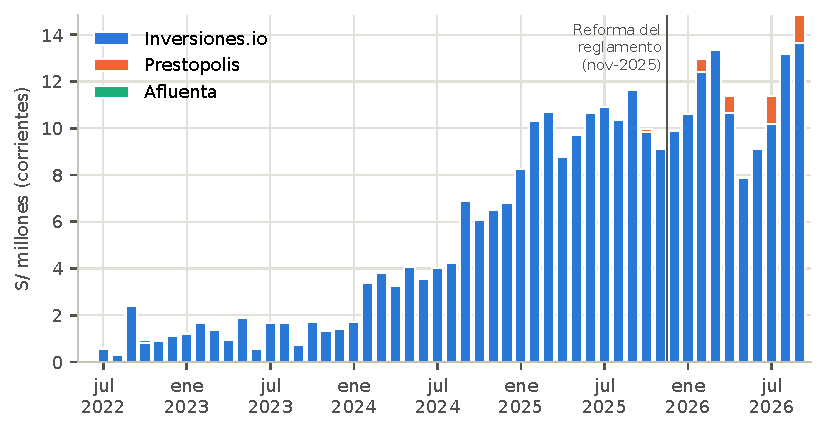
\includegraphics[width=\linewidth]{f1_monto_mensual_por_plataforma.pdf}\par
\captionof{figure}{\cifra{tituloF1}. Datos de la SMV (SIMV).}\par}

{\small\centering
\begin{tabularx}{\linewidth}{@{}X>{\raggedleft\arraybackslash}p{4.6cm}>{\raggedleft\arraybackslash}p{4.6cm}@{}}
  \toprule
  Indicador & 2022 & 2025 \\
  \midrule
  Monto financiado (S/ millones) & \cifra{monto2022} & \cifra{monto2025} \\
  Proyectos financiados & \cifra{proyFin2022} & \cifra{proyFin2025} \\
  Monto medio por proyecto (S/ miles) & \cifra{montoMedio2022} & \cifra{montoMedio2025} \\
  Tasa de colocación (\%) & \cifra{colocacion2022} & \cifra{colocacion2025} \\
  IHH & \cifra{hhi2022} & \cifra{hhi2025} \\
  \bottomrule
\end{tabularx}
\captionof{table}{Indicadores clave de la oferta}\par}

\textbf{Plataformas.} La líder cerró 2025 con activos de S/~\cifra{activoLider2025} mil y un ROA anualizado de \dato{\cifra{roaLider2025}~\%}; las demás perdieron en \cifra{aniosOtrasPerdida} de \cifra{aniosOtras} años. Sus ingresos equivalen al \dato{\cifra{costoMediana}~\%} del monto financiado: lo que retiene la plataforma, no la tasa del receptor.

\textbf{Acceso (H2).} Colocación de \cifra{colocacionEmp}~\% en proyectos empresariales y \cifra{colocacionPer}~\% en personales ($z=\cifra{hDosZ}$), pero cada tipo se concentra en una plataforma: dentro de la líder la diferencia no es significativa (Fisher, $p\cifra{hDosFisherPRel}$).

\textbf{Reforma (H1).} La mediana mensual subió de S/~\cifra{hUnoMedianaAntes} M a S/~\cifra{hUnoMedianaDespues} M ($p\cifra{hUnoPRel}$), pero los \cifra{placeboN} cortes ficticios previos también son significativos y el crecimiento interanual bajó de \cifra{interanualAntes}~\% a \cifra{interanualDespues}~\%: la diferencia no es atribuible a la norma.

{\centering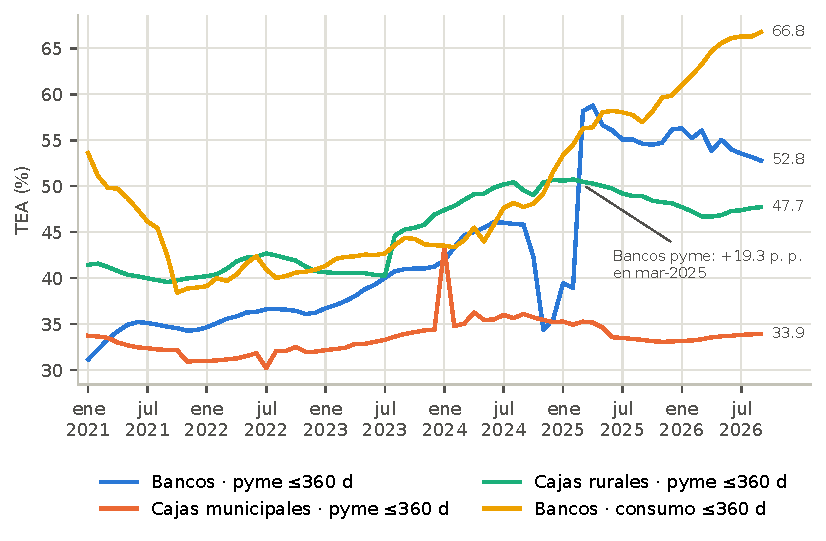
\includegraphics[width=\linewidth]{f3_tasas_credito_tradicional.pdf}\par
\captionof{figure}{\cifra{tituloF3}. Datos del BCRP (BCRPData).}\par}

\textbf{Crédito tradicional (E1).} Las tasas son altas y la bancaria pyme saltó \cifra{saltoTEA} p.~p. en marzo de 2025; los cambios del FPF no se asocian con los de las tasas (\cifra{eUnoN} comparadores, $p_{\min}=\cifra{eUnoPMin}$). Sin tasa ni plazo por operación, \textbf{el precio del FPF no es comparable}.

% ---------------------------------------------------------------- Conclusiones
\vspace{0.8em}
\begin{tcolorbox}[enhanced, colback=primarioclaro, colframe=primarioclaro, boxrule=0pt, arc=0pt, left=14pt, right=14pt, top=12pt, bottom=14pt]
  \refstepcounter{seccion}{\color{primario}\bfseries\fontsize{44}{51}\selectfont\theseccion.\hspace{0.45em}Conclusiones\par}
  \vspace{0.4em}
  \begin{enumerate}
    \item El FPF creció de S/~\cifra{monto2022} M a S/~\cifra{monto2025} M al año, pero \textbf{una plataforma concentra casi todo}.
    \item Es un mercado de \textbf{préstamos a empresas} con montos crecientes; solo la plataforma líder es rentable.
    \item Las diferencias por receptor reflejan el \textbf{modelo de negocio}, y el aumento tras 2025 \textbf{no es atribuible} a la norma.
    \item Sin tasa ni plazo por operación \textbf{no puede compararse el precio}: la SMV debería publicarlos.
  \end{enumerate}
\end{tcolorbox}

% ---------------------------------------------------------------- Fuente de datos y repositorio
\seccion{Fuente de datos y repositorio}
{\footnotesize\RaggedRight
\fullcite{bcrpdata2026}\par\vspace{0.4em}
\fullcite{smvodata2026}\par\vspace{0.4em}
\fullcite{smvsimv2026}\par}
\vspace{0.6em}
\begin{minipage}[c]{0.38\linewidth}\centering\qrcode[height=6.2cm]{\repositorio}\end{minipage}\hfill
\begin{minipage}[c]{0.58\linewidth}\RaggedRight\small
  \textbf{Repositorio de extracción}: código en Python (API y \textit{scraping}), datos crudos y procesados, tablas, figuras y artículo.\par\vspace{0.3em}
  {\footnotesize\url{https://github.com/Diego-Aliaga-Damian/finanzas1-u2-crowdfunding-peru}}
\end{minipage}
\end{multicols}

\vfill
{\color{gris}\hrule height 1.2pt}
\vspace{0.3em}
{\scriptsize\centering Las cifras y figuras se generan con el código del repositorio a partir de los datos oficiales de la SMV y del BCRP. Elaborado con apoyo de herramientas de inteligencia artificial (ver la declaración del artículo).\par}
\end{document}
